\chapter{Introducción}

% Especifica donde se encuentras las figuras
\ifpdf
    \graphicspath{{1_introduction/figures/PNG/}{1_introduction/figures/PDF/}{1_introduction/figures/}}
\else
    \graphicspath{{1_introduction/figures/EPS/}{1_introduction/figures/}}
\fi

%: --------------------------------------------------------------
%:                          Introducción
% -------------------------------------------------------------- 
El cáncer de piel es una enfermedad de carácter más o menos grave, según el tipo de tumor al que dé lugar.
El melanoma es un tipo de cáncer de piel que se origina cuando los melanocitos \ref{skin} (las células responsables de la pigmentación normal de la piel) comienzan a crecer fuera de control \cite{cancer-org}. Este es mucho menos frecuente que otros tipos de cánceres de piel, aunque es el más peligroso y agresivo debido a que evoluciona muy rápidamente, es de fácil diseminación por el organismo y muchas veces mortal si no es detectado en una fase temprana.

\begin{figure}[htbp]
    \centering
    \textbf{}\par\medskip
    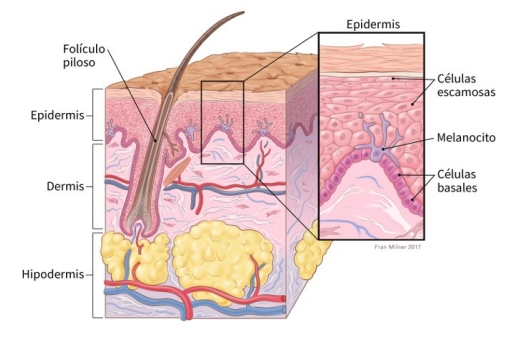
\includegraphics[scale=0.65]{skin.png}
    \caption{Capas de la piel \cite{cancer-org}}
    \label{skin}
\end{figure}

Muchos tipos de tumores benignos (no cancerosos) se pueden originar de los diferentes tipos de células de la piel. Un lunar es un tumor benigno de la piel que también se origina a partir de los melanocitos. No obstante, casi todos los lunares son inofensivos, aunque algunos tipos pueden aumentar su riesgo de melanoma. 

Un tipo de lunar que a veces se parece al melanoma se llama “nevo Spitz”. Este lunar es más común en niños y adolescentes, aunque a veces se presenta en adultos. Por lo general, estos tumores son benignos y no se propagan. Sin embargo, en ocasiones los médicos tienen problemas para distinguir entre un “nevo Spitz” y un melanoma, aun cuando los observan con un microscopio.

\newpage

En general, las variedades de melanoma se caracterizan por su Asimetría, Borde irregular, Color heterogéneo, Diámetro grande ($>$ 6mm) y Evolución rápida, también conocido como la regla del ABCDE.
Se reconocen actualmente como factores de riesgo de melanoma:

\begin{table}[htb]
\centering
%\small
\begin{tabular}{*{2}{p{.425\linewidth}}}
\midrule
Factores personales & 
Características fenotípicas: piel y ojos claros, pelo rubio o pelirrojo, presencia de efélides y tendencia a quemarse fácilmente y a no pigmentarse o hacerlo con dificultad tras la exposición al sol.

Antecedentes familiares de melanoma y de síndrome del nevus displásico familiar.

Tener un elevado número de nevi benignos (mayor que 50).

Presencia de nevi congénito grande o gigante.

Otros: Xeroderma pigmentoso (padecimiento hereditario que afecta a la capacidad de las células de la piel de reparar el daño causado a su ADN), Inmunodepresión (síndromes linfoproliferativos, VIH, inmundeficiencias primarias, transplantados que están con tratamiento inmunosupresor...).\\

\midrule % the p{} setting automatically lets these be multi-line - we don't want multiple rows on top of that and this is simpler as TeX does the hard work for us

Factores ambientales & 
Radiación Ultravioleta, que es el factor etiopatogénico más importante en el desarrollo del melanoma cutáneo. \\
\bottomrule
\end{tabular}
\captionof{table}{Factores de riesgo de melanoma \cite{pediatriaintegral}}
\end{table}

Según la etapa del cáncer y otros factores, las opciones de tratamiento podrían incluir: cirugía, inmunoterapia, medicamentos de terapia, quimioterapia, radioterapia para el cáncer de piel tipo melanoma, entre otros.

\newpage
%: --------------------------------------------------------------
%:                           Motivación
% --------------------------------------------------------------
\section{Motivación} 
El cáncer de piel está aumentando en muchos países, debido a que cada vez la capa de ozono que protege a la tierra de la radiación solar se debilita. Uno de los principales responsables del cáncer de piel de melanoma es la radiación ultravioleta proveniente del sol, o de cualquier otra fuente artificial de radiación ultravioleta, como las lámparas bronceadoras \cite{uvi}.

El Índice de Radiación Ultravioleta (Índice UV o UVI) se mide en una escala a partir de 0 sin límite superior, en la que un índice UV menor de 2, representa un riesgo bajo (código de color verde) y un índice UV mayor de 11 representa un riesgo extremadamente alto (código de color violeta).

En Canarias, no solo el sol acompaña todo el año con una exposición constante, también una exposición estacional; es decir, personas que durante todo el año no toman demasiado sol pero que en verano sí lo hacen de forma constante. Al sol de Canarias también se suman los niveles de radiación que existe en la región dada su proximidad al Ecuador. Esto hace que el índice de radiación UV sea extremadamente elevado \ref{indice_uv}, siendo el más alto de las Comunidades Autónomas de España.
%\newpage

\begin{figure}[htbp]
    \centering
    \textbf{}\par\medskip
    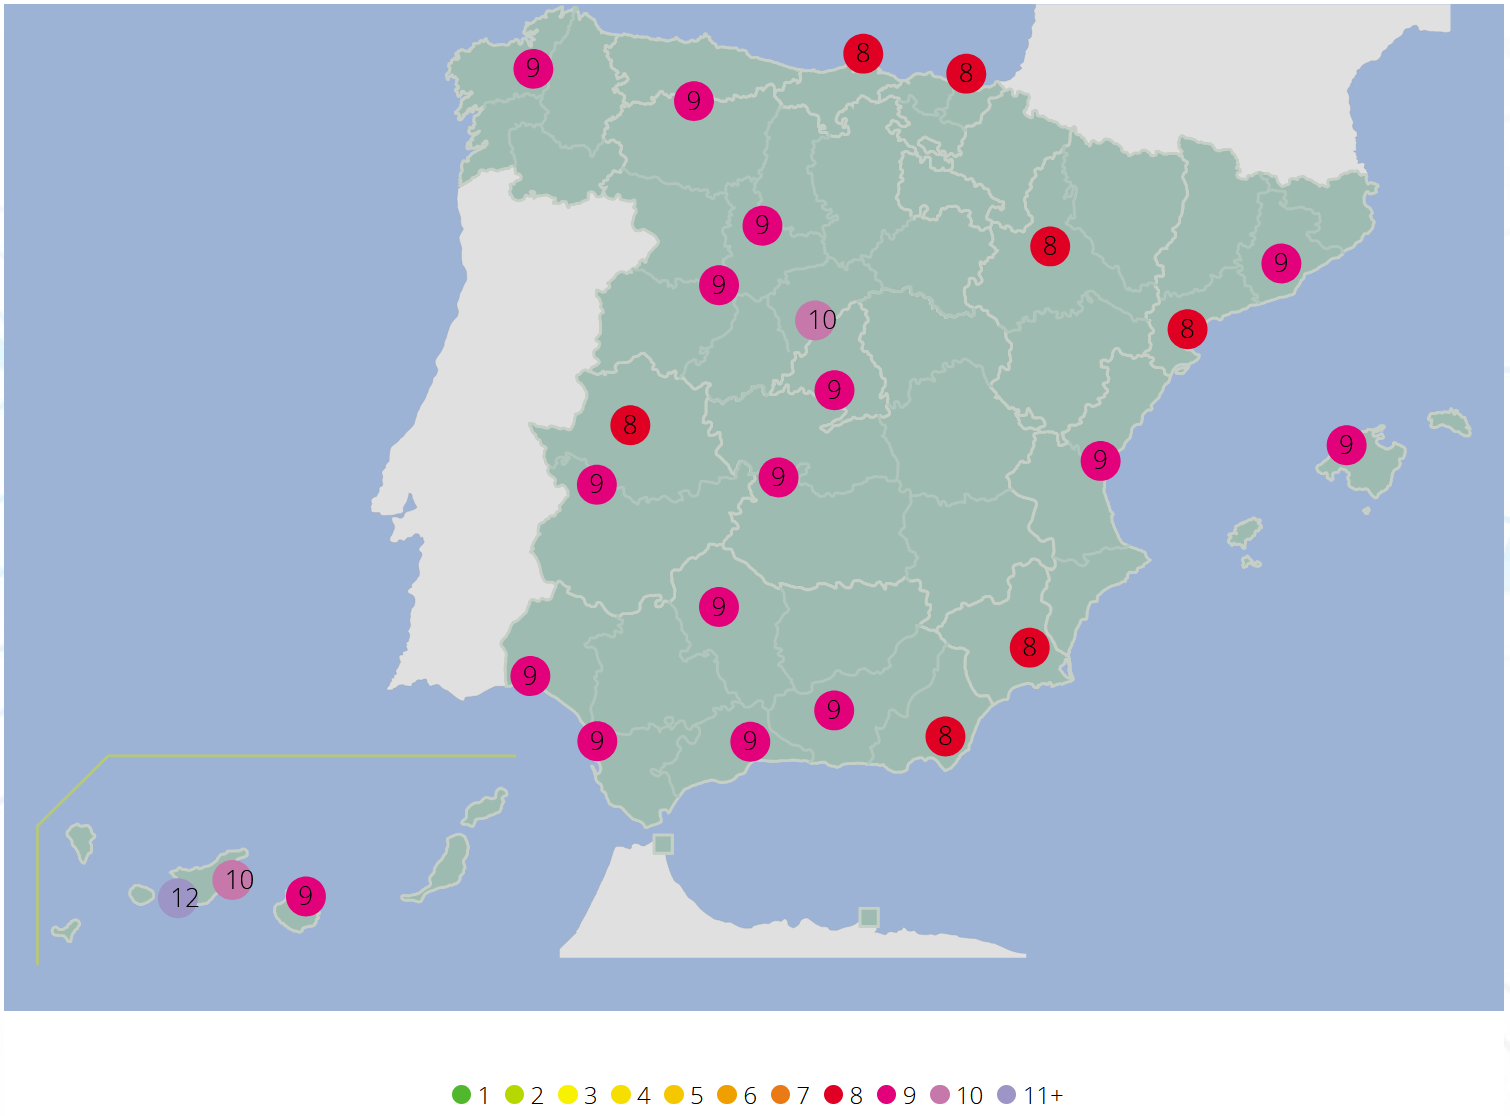
\includegraphics[scale=0.45]{indice_uv.png}
    \caption{Índice UV de las Comunidades Autónomas de España (datos del sábado, 17 julio 2021) \cite{uvi}}
    \label{indice_uv}
\end{figure}

%\bigskip
Por lo que, la motivación principal del trabajo ha sido la identificación e incorporación de los factores que influyen en el cáncer de piel para obtener el valor predictivo positivo a partir de dichos factores y del resultado de un clasificador basado en redes neuronales convolucionales.

%: --------------------------------------------------------------
%:                           Estado del arte
% --------------------------------------------------------------
\section{Estado del arte} 
...

%: --------------------------------------------------------------
%:                           Objetivos
% --------------------------------------------------------------
\section{Objetivos} 
El objetivo principal es apoyar el diagnóstico médico, ayudar a los médicos para tomar mejores decisiones y detectar la enfermedad en una fase tempranera con el propósito de poder realizar el tratamiento adecuado. Para ello se implementa un clasificador capaz de discernir imágenes de cáncer maligno (particularmente, de tipo melanoma) y benigno a partir de un conjunto de datos desbalanceados. Asimismo, implementar una red bayesiana que permita identificar e incorporar otros factores que influyen en el cáncer de piel.

%: --------------------------------------------------------------
%:                           Metodología
% --------------------------------------------------------------
\section{Metodología}
El desarrollo se ha hecho principalmente en la plataforma de Kaggle utilizando Jupyter Notebook, en el lenguaje de programación Python.

\bigskip

%: --------------------------------------------------------------
%:                   Tabla de modelos con métricas
% --------------------------------------------------------------
%\begin{table}[htp]
%\centering
%\begin{tabular}{ccc} 
%
%{\bf Descripción de modelos} & {\bf  Métrica 1 } & {\bf Métrica 2} \\ 
%\hline
%
%Modelo 1  & item 22  & item 23 \\
%Modelo 2  & item 22  & item 23 \\
%Modelo 3  & item 22  & item 23 \\
%
%\end{tabular}
%\caption[title of table]{\textbf{title of table} - Overview of latexin %genes.}
% You only need to write the title twice if you don't want it to appear in %bold in the list of tables.
%\label{latexin_genes} % label for cross-links with \ref{latexin_genes}
%\end{table}


%: ----------------------- HELP: references
% References can be links to figures, tables, sections, or references.
% For figures, tables, and text you define the target of the link with \label{XYZ}. Then you call cross-link with the command \ref{XYZ}, as above
% Citations are bound in a very similar way with \cite{XYZ}. You store your references in a BibTex file with a programme like BibDesk.

%\figuremacro{largepotato}{A common glucose polymers}{The figure shows starch %granules in potato cells, taken from %\href{http://molecularexpressions.com/micro/gallery/burgersnfries/burgersnfr%ies4.html}{Molecular Expressions}.}

%: ----------------------- HELP: adding figures with macros
% This template provides a very convenient way to add figures with minimal code.
% \figuremacro{1}{2}{3}{4} calls up a series of commands formating your image.
% 1 = name of the file without extension; PNG, JPEG is ok; GIF doesn't work
% 2 = title of the figure AND the name of the label for cross-linking
% 3 = caption text for the figure

%: ----------------------- HELP: www links
% You can also see above how, www links are placed
% \href{http://www.something.net}{link text}

%\figuremacroW{largepotato}{Title}{Caption}{0.8}
% variation of the above macro with a width setting
% \figuremacroW{1}{2}{3}{4}
% 1-3 as above
% 4 = size relative to text width which is 1; use this to reduce figures